\subsection{Dust properties of the nucleus}
\label{sect:nucleus}

\begin{figure}
\centering
\caption{Here is where we show the PAHFIT analysis of the nucleus spectrum.}
\label{fig:nuc_pahfit}
\end{figure}


The extracted IRS spectrum of the M31 nuclear region (Figure~\ref{fig:nuc_pahfit})
looks different from most of the other spectra, with
a blue continuum, PAH features weak or absent at 6--8~$\mu$m  but detectable at 11.3~$\mu$m.
{\bf NEED some further discussion of the nuclear spectrum in general here.}
Figure \ref{nuc11} (top) shows the integrated intensity map of 11.3~$\mu$m emission around the nucleus. The majority of the 11.3~$\mu$m 
emission is from a region 15\arcsec\ north of the nucleus and not from the nucleus itself. 
On the other hand, the centre shows no PAH emission,  but it does have silicate emission around 9.7~$\mu$m, 
which comes only from the nucleus and is not present in the North spectrum 
(see Figure \ref{nuc11}, bottom panel).
Both the 11.3~$\mu$m  and silicate emission sources are consistent with being unresolved point sources.
We extracted spectra from the centre and the North regions using  $9\arcsec \times 9\arcsec$ 
square apertures as shown in Figure \ref{nuc11}. 

% SPW had some comments on number of ticks in these -- prob going to ignore
\begin{figure}
\centering
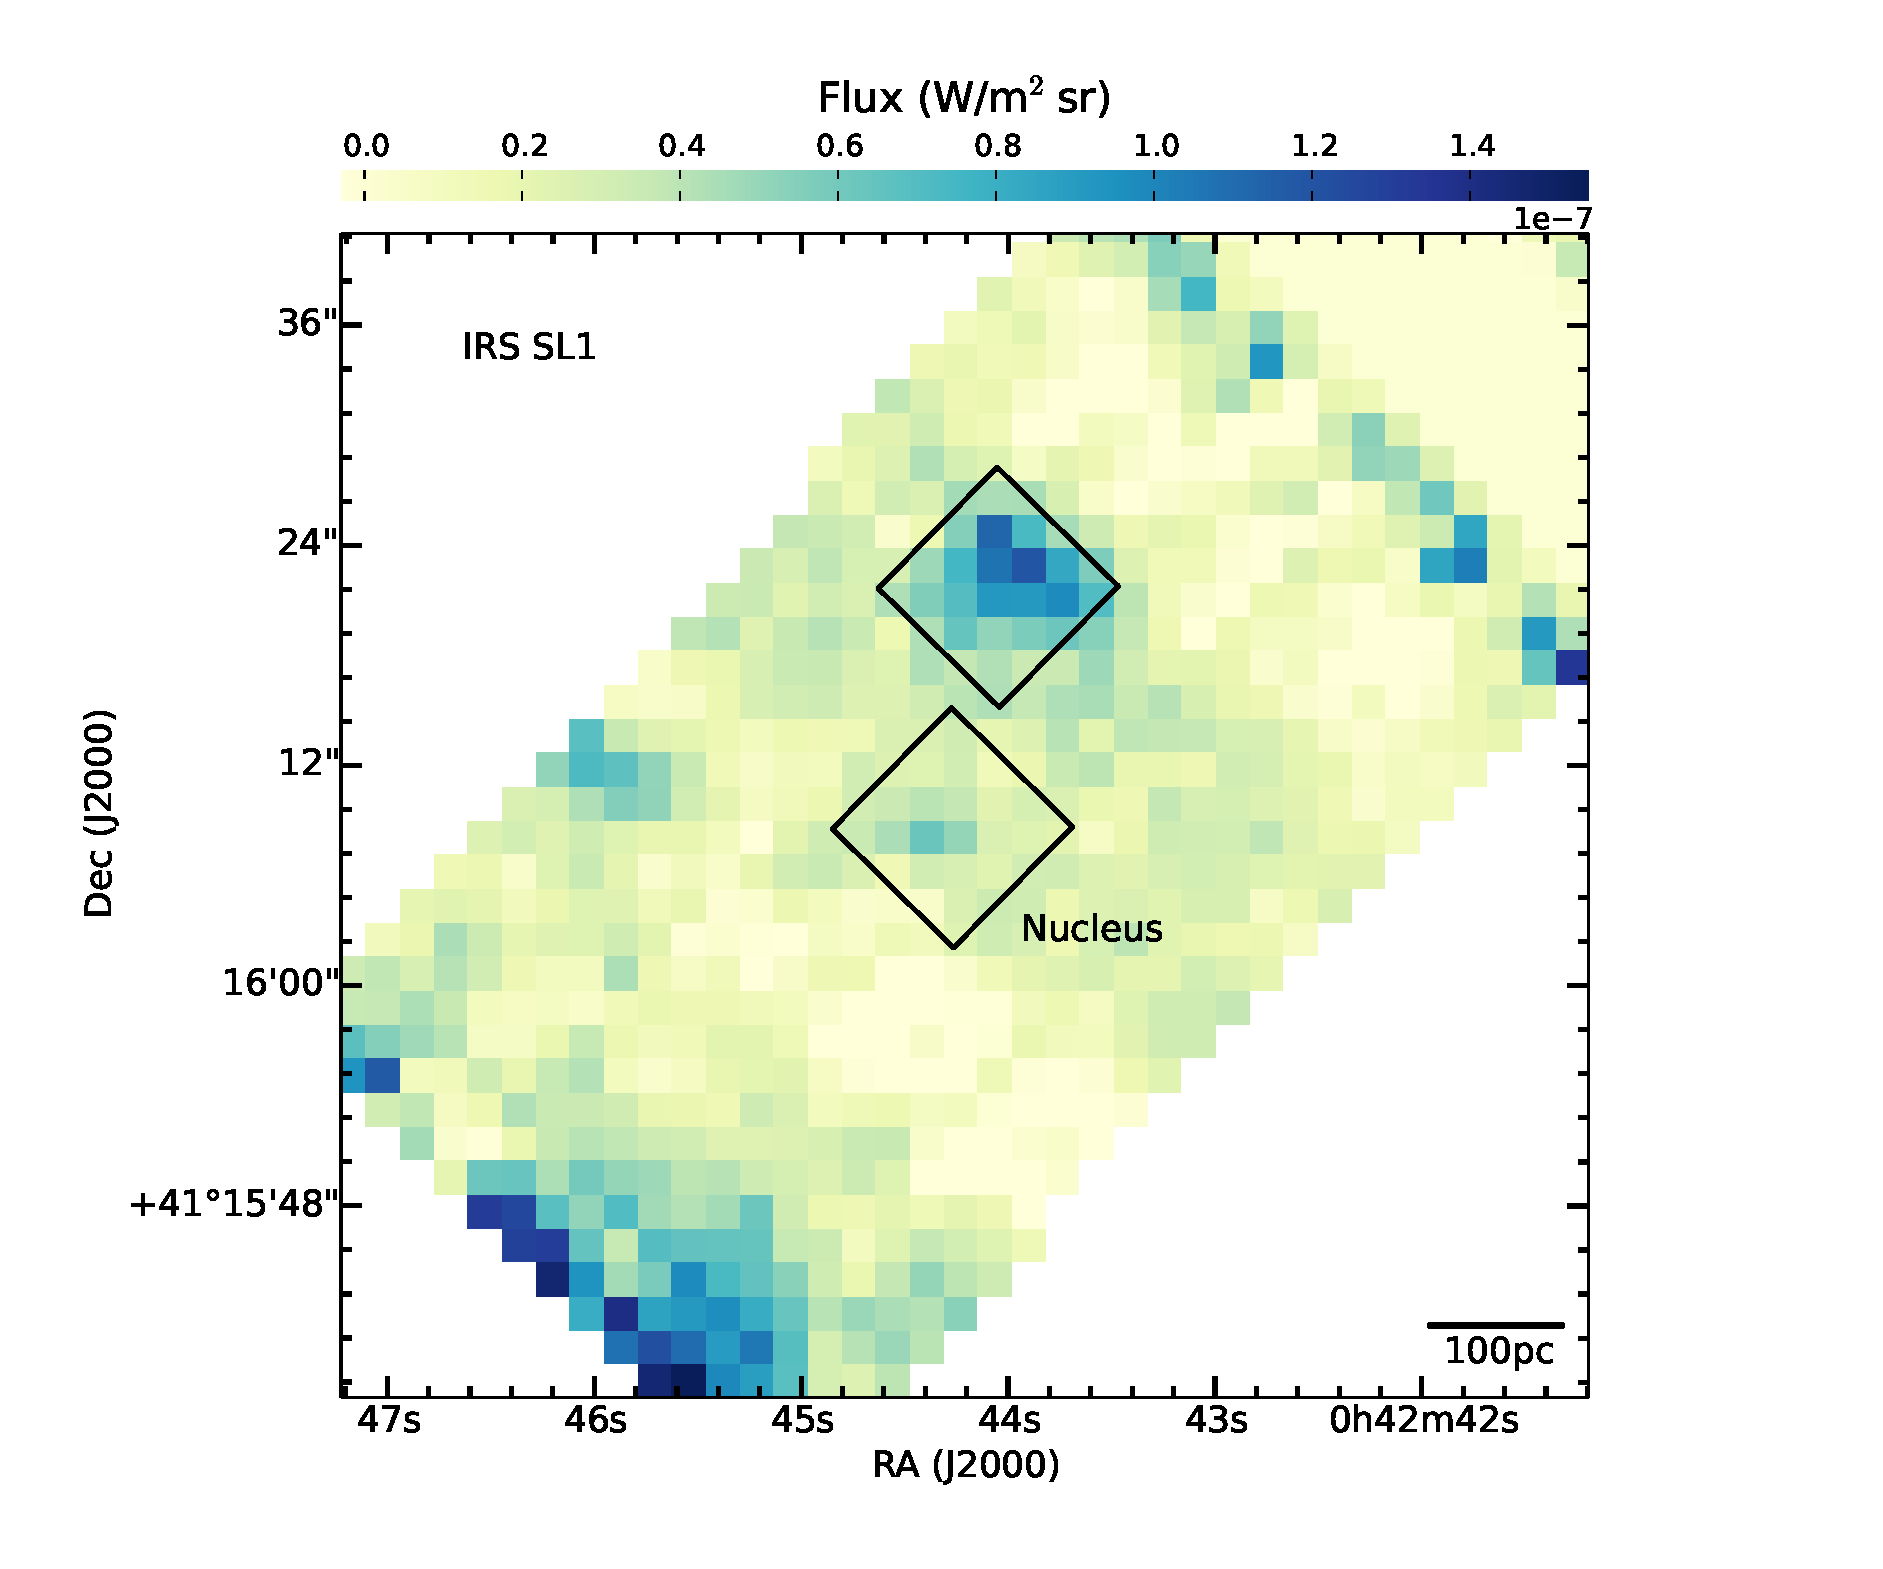
\includegraphics[width = 8 cm]{./nuc11_3.eps}
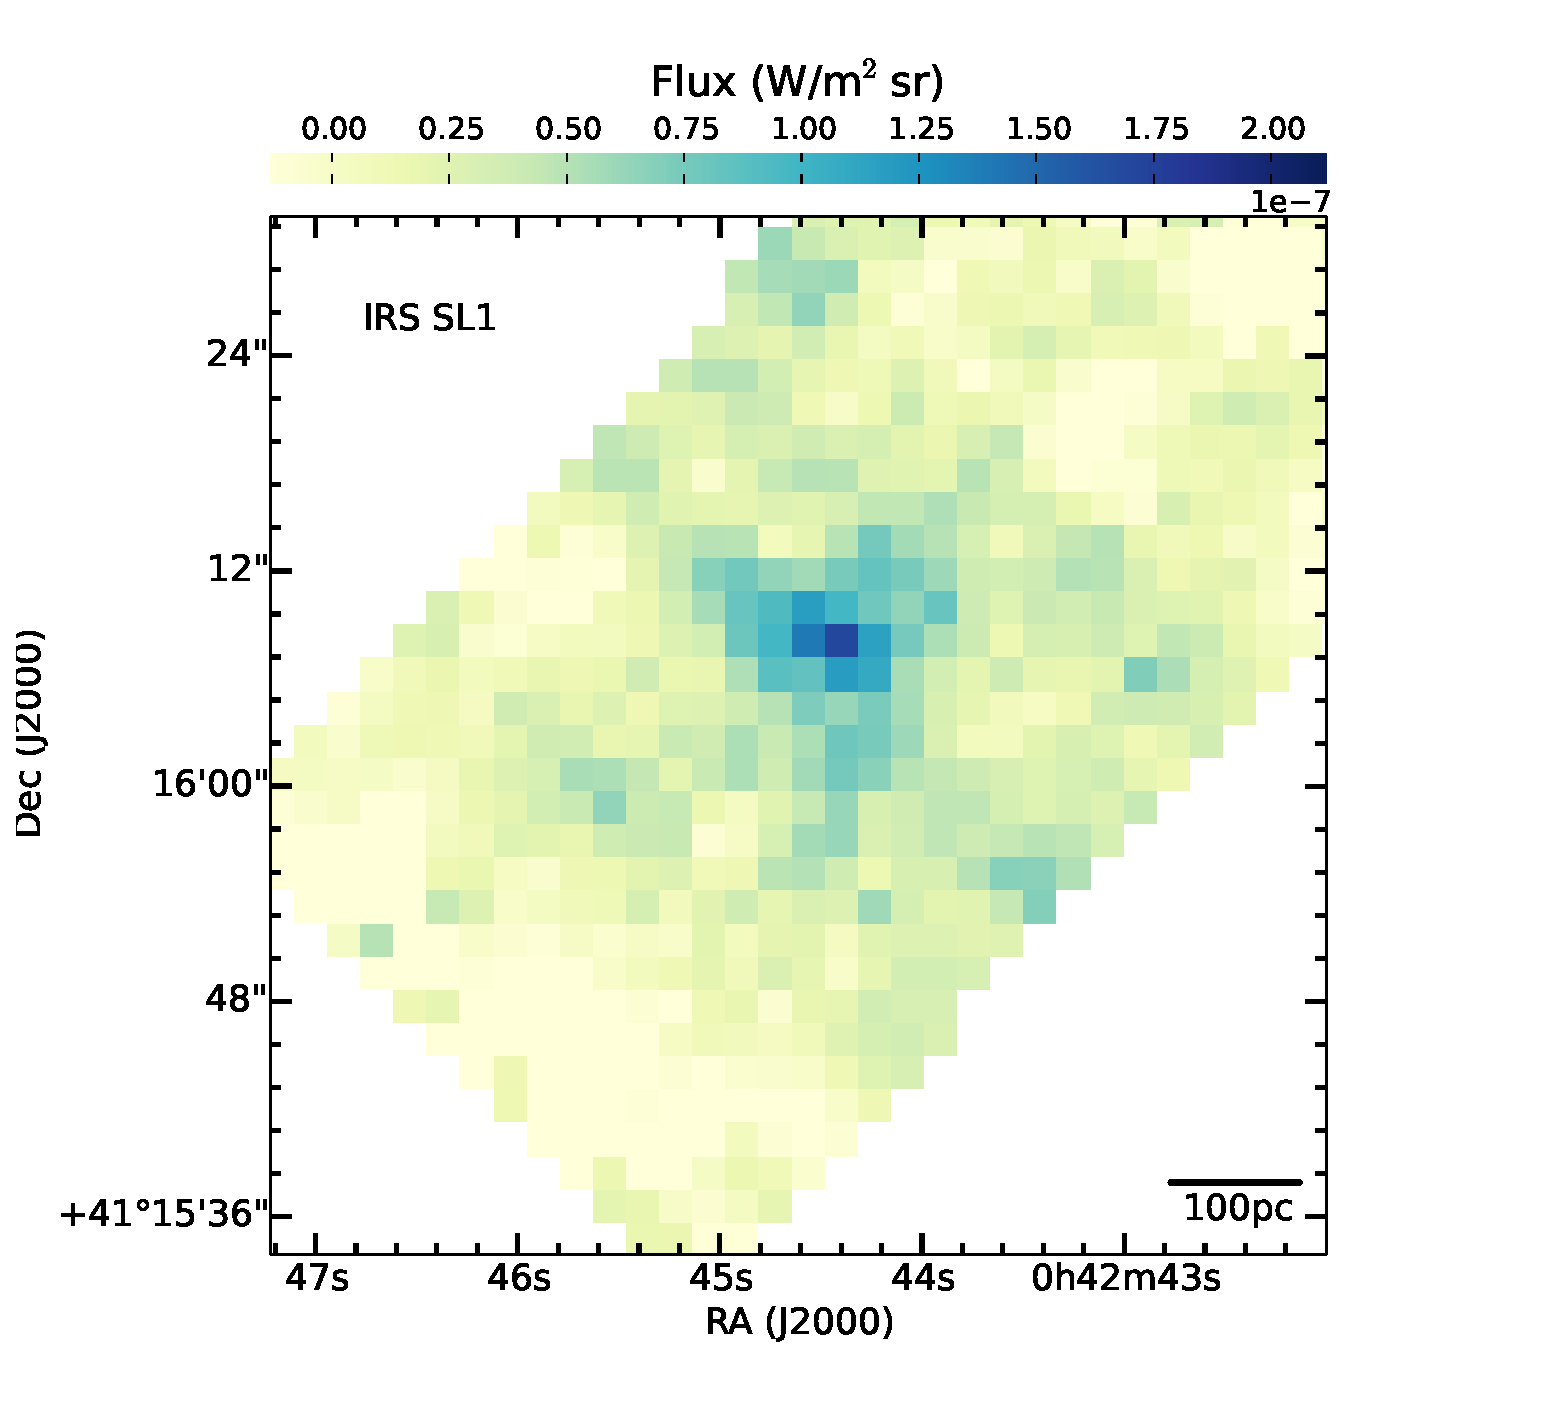
\includegraphics[scale = 0.3]{./NUCsilicate.eps}
\caption{(Top): Intensity variation of 11.3~$\mu$m emission around the nucleus of M31. 
Two black boxes are the apertures (centre and north region) used to extract spectra in Figure \ref{smithspec}. 
The centre of the nucleus is at R.A. $00^{\rm h}42^{\rm m}44\fs35$, Dec. $+41\degr16\arcmin08\farcs5$ \citep{NucleusREF}. % TODO: mark in figure. Is this the stellar centre?
(Bottom:) Integrated strength of the silicate emission (from 9 to 11~$\mu$m, continuum subtracted) near the M31 nucleus.} % CHECK - is this continuum subtracted?
\label{nuc11}
\end{figure}




%
%I guess the nuclear spectrum is in your Figure 15 - why did you not try to fit it with PAHFIT too?  It looks to me like it has a weak 20um silicate bump too.
% Why not include the nuclear region in Tables 2,3&4?  I did not understand the reason for leaving it off.  Also please add the limit for the [Ne V] detection - it might still be a useful ratio with [Ne II] and the PAH lines.  It looked to me like there was some hint of the H2 12.28um line in some regions.... maybe add that limit too, though I was surprised

\begin{figure*}
\centering
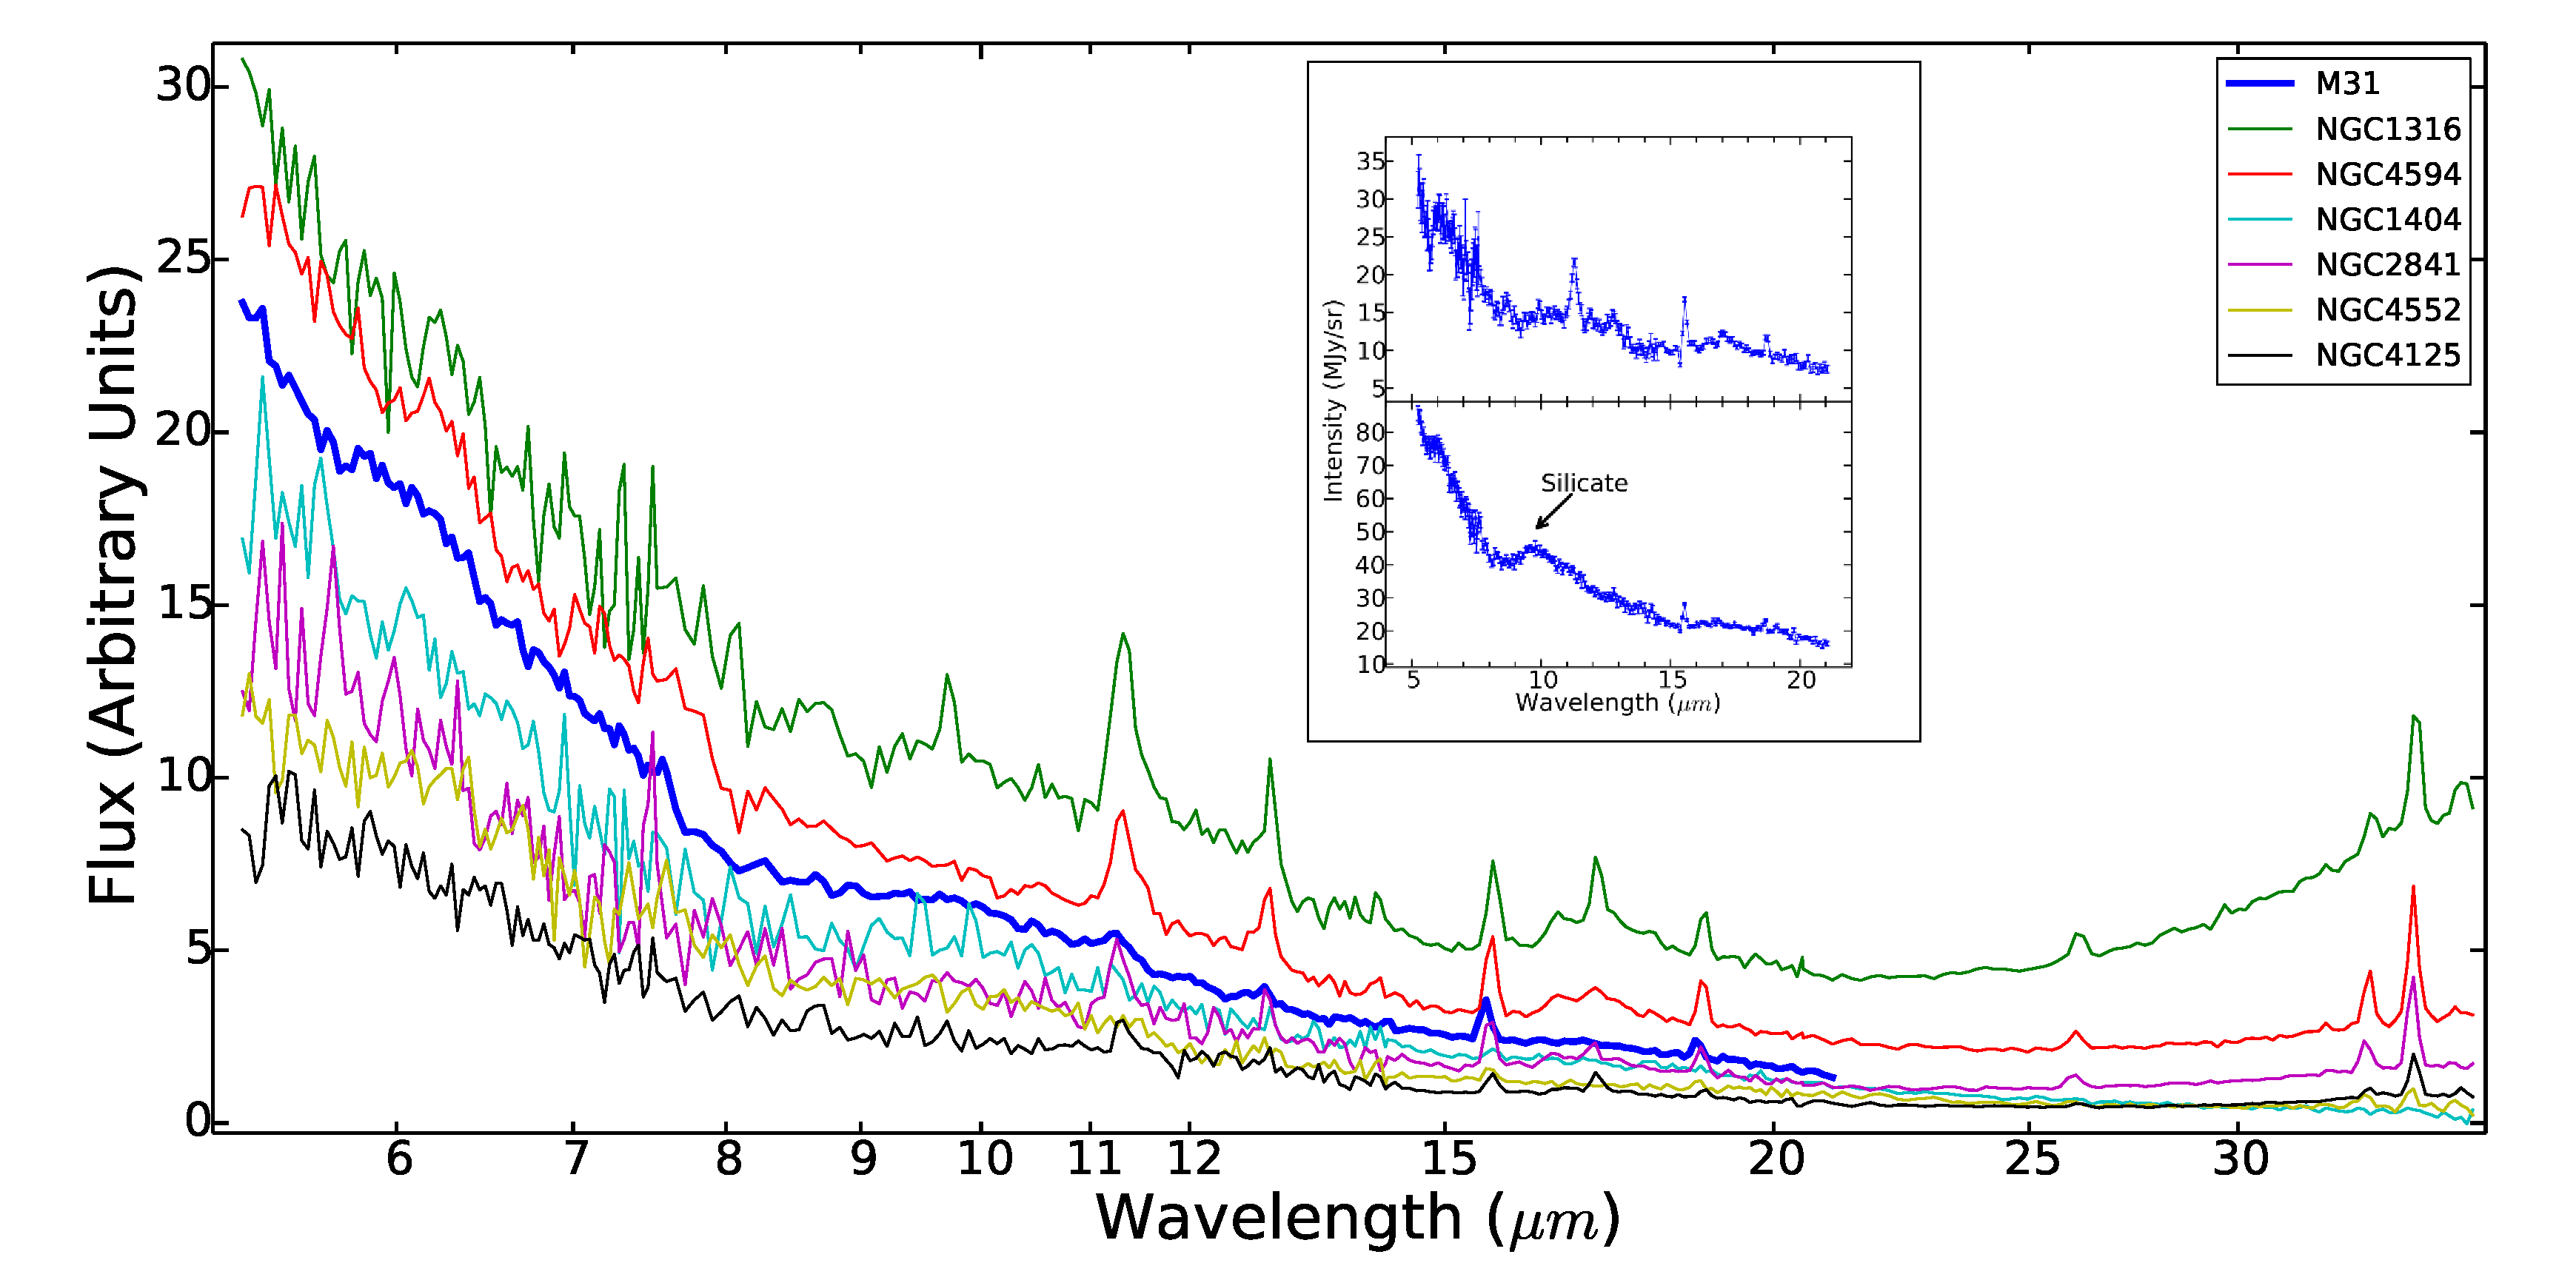
\includegraphics[height = 8 cm]{./SINGSspec.eps}
\caption{Mid-infrared spectrum of the nucleus of M31 (blue) over-plotted with spectra extracted close to the nuclei of 6 nearby galaxies which have 
AGN activity \citep{Smith:2007lr}. NGC 4552, NGC 1404 and NGC 4125 are elliptical galaxies and NGC 4594 and NGC 2841 are spiral galaxies. 
NGC 1316 is a lenticular galaxy. The inset shows the spectra extracted from the centre region of the M31 nucleus (bottom) and from the north region (top) 
shown in Figure \ref{nuc11}.}
\label{smithspec}
\end{figure*}

The mid-infrared spectra of the nucleus from both {\em Spitzer} and ISOCAM (Figure~\ref{ISOnIRS}) show similar characteristics: a blue
continuum, PAH features weak or absent at 6--8~$\mu$m  but detectable at 11.3~$\mu$m, and detectable atomic fine structure lines.
Comparing the M31 nuclear spectrum with the nuclear spectra from the SINGS sample given by \citet{Smith:2007lr}, we found
six other galaxies with similar spectral shapes, including three elliptical galaxies, two spirals, and a lenticular.%
\footnote{The IRS spectra for the SINGS galaxies were extracted over areas ranging from 2 to 8 kpc$^2$, whereas the M31
nucleus spectrum covers a much smaller area (0.02~kpc$^2$).}
Published estimates of the black hole masses for these galaxies range from $1.5-5.5\times10^{8}$~M$_{\sun}$
\citep[for NGC~1316 and NGC~4595, respectively]{nowak08, kormendy88}, or about $1-4\times$ that of M31.
The SINGS papers \citep{kennicutt03,Smith:2007lr, moustakas2010} are in some disagreement over the
exact nuclear spectral types of these six galaxies. All are classified as some form of low-luminosity AGN
such as Seyfert or LINER \citep[luminous AGNs were intentionally omitted from the SINGS sample;][]{kennicutt03}, but they are
by no means the only LLAGN in the SINGS sample.
In contrast with the nuclear spectrum, the spectrum extracted from the North region (offset by 15\arcsec from the center; 
Figure \ref{smithspec}, inset) shows a strong 11.3~$\mu$m peak 
and no significant emission from 6--8~$\mu$m features. These characteristics are shared by
the M81 nuclear spectrum presented by \citet{Smith2010}, although that spectrum has little stellar continuum and a very strong [Ne {\sc ii}]~12.8~$\mu$m line. 


As discussed by  \citet{Smith:2007lr} and \citet{Smith2010}, inferring the suppression of 6--8~$\mu$m PAH features compared
to the 11.3~$\mu$m feature must be done with caution, because the 6--8~$\mu$m features are more susceptible to dilution by the stellar
continuum. Such suppression could have several causes: destruction of small or charged PAH molecules by an AGN,
or weak ultraviolet continuum indicating lack of star formation \citep{Smith:2007lr}. In the latter case, the AGN is not the cause of
the suppressed  6--8~$\mu$m features but rather is only detected when the nuclear star formation rate is low.
Low rates of star formation in the centre of M31 are consistent
with previous work: although \citet{Melchior2013} found a significant amount of cold gas in the centre of the galaxy, this gas does not
appear to be associated with current star formation. In modelling the far-infrared spectral energy distribution, \cite{Groves2012} found that  
the old stellar population in the M31 bulge is sufficient  to heat the observed dust; no young stellar population is needed.


Examining the spatial distribution of the mid-infrared emission in the M31 nuclear region provides additional clues
to the nature of the emitting sources. Figure~\ref{nuc11} shows that most of the 11.3~$\mu$m comes from a region to the
north of the nucleus, while the silicate emission (Figure~\ref{nuc11},  bottom) is centred on the nucleus itself.  
Figure \ref{smithspec} compares the spectra extracted from these two regions. % need to say something about the figure!
Silicate emission is not very common in
integrated spectra of galaxies \citep{Spoon2007} but is seen in luminous quasar spectra \citep{Hill14} and, as mentioned above, in the
spectrum of the M81 nucleus. We computed the linear slope parameter  defined by \citet{Smith2010},
$\gamma810 =[F_{\nu}(10\mu{\rm m}) -F_{\nu}(8\mu{\rm m})]/2F_{\nu}(9\mu{\rm m}) $, for the M31 nucleus and
found $\gamma810 =-0.08\pm 0.06$.  This is  to be completed % TBD

Does detection of silicate emission in the M31 nuclear spectrum imply the detection of an active nucleus?
In the unified model of AGNs, an obscuring torus viewed face-on would be expected to show silicate emission
\citep{AGNtypes1995, AGNref}; however such a view would also be expected to show forbidden atomic lines such as [Ne~{\sc v}] and [S~{\sc iv}],
not seen in the M31 spectrum. Alternatively, \citet{Mason2012} explained that low-luminosity AGNs cannot 
host a Seyfert-like obscuring torus because of their optically thin dust and low dust-to-gas ratio but can show
the silicate emission that originates in the optically thin hot dust around the torus.  The first detection of such silicate emission was 
reported by \citet{Sturm2005} from the low-ionization nuclear emission-line region (LINER) galaxy NGC~3998, and 
\citealt{Mason2012}  observed that this 9.7~$\mu$m silicate emission is present in many LLAGNs. 
The IRS spectrum of the M31 nucleus has a 12~$\mu$m flux  of XX; using the method described by \citet{luminosity}
the  bolometric luminosity of the M31 nucleus is inferred to be (**value goes here**) erg~s$^{-1}$ .
 This value is close to that of other LLAGNs (**and consistent with the X--ray value?**)
